\documentclass{article}

\usepackage{graphicx}
\usepackage[margin=1in]{geometry}
\usepackage{listings}
\lstset{
basicstyle=\small\ttfamily,
columns=flexible,
breaklines=true
}
\usepackage{hyperref}

\begin{document}

% latex table generated in R 4.3.2 by xtable 1.8-4 package
% Tue Aug 27 21:46:35 2024
\begin{tabular}{cccc}
  \hline
5-digit ZIPs Excluded by LPW & Treated in OK (2022) & State FIPS & Hurricane in OK (2022) \\ 
  \hline
70615 & Yes & 22 & RITA 2005 \\ 
  77702 & Yes & 48 & RITA 2005 \\ 
  21085 & Yes & 24 & SANDY 2012 \\ 
  11096 & Yes & 36 & SANDY 2012 \\ 
  19703 & Yes & 10 & SANDY 2012 \\ 
  10474 & Yes & 36 & SANDY 2012 \\ 
  21017 & Yes & 24 & SANDY 2012 \\ 
  10303 & Yes & 36 & SANDY 2012 \\ 
  70094 & Yes & 22 & KATRINA 2005 \\ 
  39576 & Yes & 28 & KATRINA 2005 \\ 
  70094 & Yes & 22 & GUSTAV 2008 \\ 
  77702 & Yes & 48 & IKE 2008 \\ 
  77530 & Yes & 48 & IKE 2008 \\ 
  77480 & Yes & 48 & IKE 2008 \\ 
  77058 & Yes & 48 & IKE 2008 \\ 
  77591 & Yes & 48 & IKE 2008 \\ 
  77506 & Yes & 48 & IKE 2008 \\ 
  23664 & Yes & 51 & IRENE 2011 \\ 
  23602 & Yes & 51 & IRENE 2011 \\ 
  23661 & Yes & 51 & IRENE 2011 \\ 
  23314 & Yes & 51 & IRENE 2011 \\ 
  27981 & Yes & 37 & IRENE 2011 \\ 
   \hline
\end{tabular}



\clearpage
\pagebreak

\begin{figure}
    
    \caption{Density of the Observations Excluded by LLPW (2024)}

    \begin{center}
        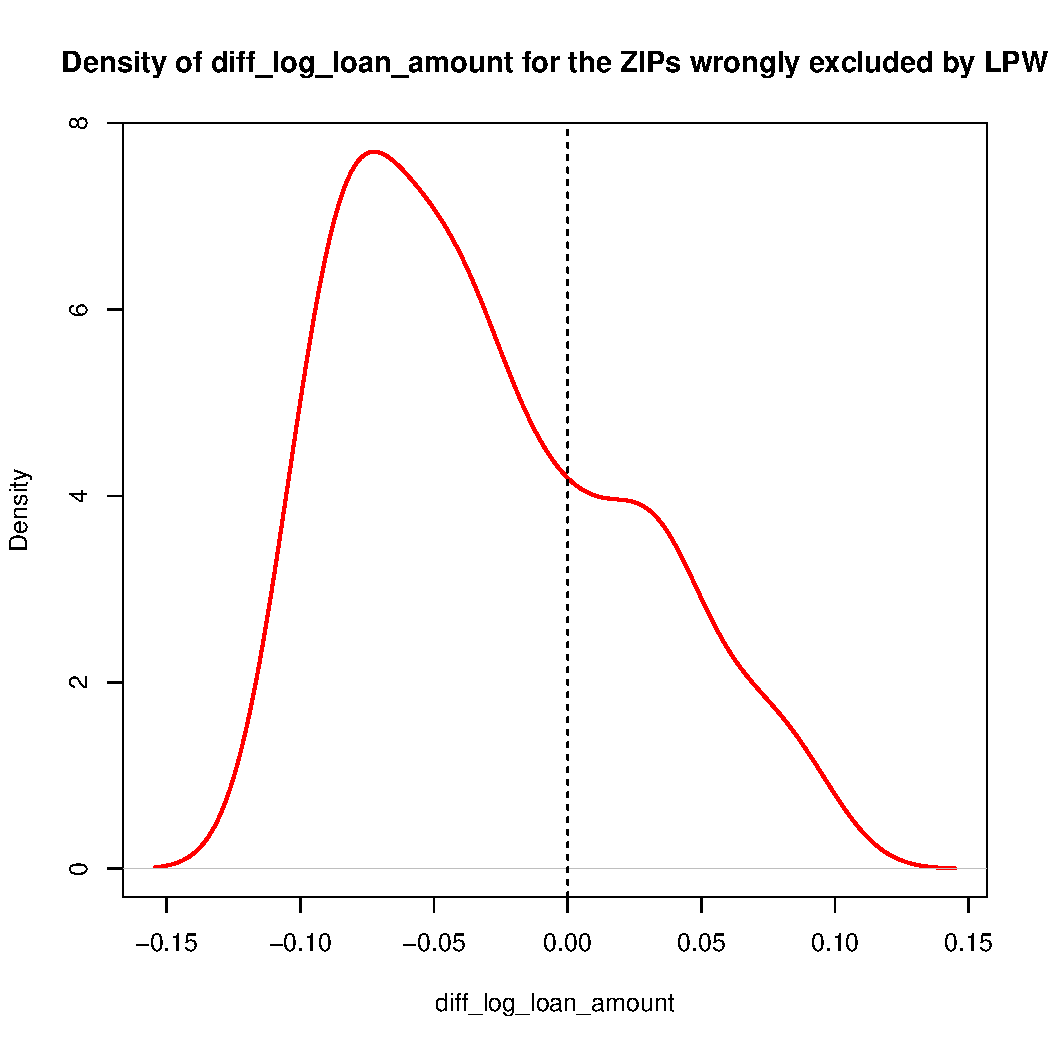
\includegraphics[scale=0.5]{figures/density_diff_log_loan_amount_excluded_ZIPs.pdf}
    \end{center}

\end{figure}

% latex table generated in R 4.3.2 by xtable 1.8-4 package
% Tue Aug 27 21:46:50 2024
\begin{tabular}{lcccccc}
  \hline
Sample & Min. & 1st Qu. & Median & Mean & 3rd Qu. & Max. \\ 
  \hline
Excluded ZIPs & -0.10 & -0.08 & -0.04 & -0.03 & 0.01 & 0.10 \\ 
  Rest of the sample & -0.11 & -0.06 & -0.01 & -0.02 & 0.00 & 0.10 \\ 
   \hline
\end{tabular}



\clearpage
\pagebreak

\begin{table}

\caption{Code that Performs Arbitrary Manipulations of the Data, Present in LLPW (2024) but not in OK (2022)}

\bigskip

\textbf{Code Evidence \#1:}

\bigskip

Code that excludes arbitrary ZIP codes on lines 140 to 143 in the RFS Dataverse code of LLPW (2024), version 1,
posted in August 2023, file \texttt{02\_generateRegressionSample.m}.

{%\footnotesize
\begin{lstlisting}
opts = detectImportOptions('excluded_ZIPs.xlsx');                                      
opts = setvartype(opts,'ZCTA5CE10','char');                                            
exclZips = readtable('excluded_ZIPs.xlsx',opts);                                       
joinedTableCombined(ismember(joinedTableCombined.ZCTA5CE10,exclZips.ZCTA5CE10),:) = [];
\end{lstlisting}}

\bigskip

\textbf{Code Evidence \#2:}

\bigskip

Code that duplicates arbitrary counties on lines 129 to 131 in the RFS Dataverse code of LLPW (2024) version 1,
posted in August 2023, file \texttt{02\_generateRegressionSample.m}.

{\footnotesize
\begin{lstlisting}
duplicateObs1 = joinedTableCombined(strcmp(joinedTableCombined.state_code,'24')&strcmp(joinedTableCombined.county_code,'510'),:);
duplicateObs2 = joinedTableCombined(strcmp(joinedTableCombined.state_code,'51')&strcmp(joinedTableCombined.county_code,'600'),:);
joinedTableCombined = [joinedTableCombined;duplicateObs1;duplicateObs2];
\end{lstlisting}}

\bigskip

\textbf{Code Evidence \#3:}

\bigskip

Code that excludes an arbitrary lender on line 134 in the RFS Dataverse code of LLPW (2024) version 1,
posted in August 2023, file \texttt{02\_generateRegressionSample.m}.

{\footnotesize
\begin{lstlisting}
joinedTableCombined(strcmp(joinedTableCombined.respondent_id,'41-1795868')&joinedTableCombined.as_of_year==2014,:) = [];
\end{lstlisting}}

\bigskip

This code can be downloaded at the RFS Dataverse, permanent DOI \url{https://doi.org/10.7910/DVN/ABVAYZ}.

\end{table}

\end{document}